\pagestyle{fancy}
\chapter{Vector Representation of Data}
\label{chap:first_chapter}

In this chapter, we will explore the field of unstructured data, discussing how it differs from the traditional structured approach and how it plays a crucial role in modern applications. We will examine the process of converting unstructured data into vectorized representation and what it entails. Additionally we will introduce Vector Database Management Systems, exploring their architecture, functionalities and their impact on the market.

\section{Unstructured Data vs. Structured Data}
In the context of data management, data can be classified as structured or unstructured. Structured data refers to information arranged in rows and columns, typically found in relational databases. These follow a defined schema and are used to store records or transactions within a database environment. Meanwhile, unstructured data lack predefined formats and cannot be easily arranged into columns. Examples include text, audio, images, documents, and videos. This characteristic makes efficient indexing, organization, and retrieval challenging.
\begin{figure}[h]
    \centering
    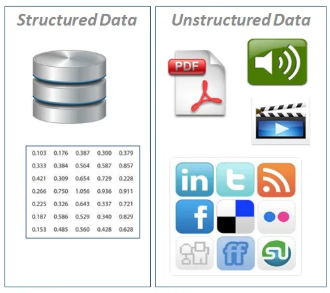
\includegraphics[width=0.4\textwidth]{IMAGES/immagine_2025-02-24_091828425.png}
    \label{fig:Structured vs. Unstructured data}
    \caption[Structured vs. Unstructured data.]{Structured vs. Unstructured data. Source: DeepLearning.AI. \footnotemark.}
    \label{fig:structuredVunstruct}
\end{figure}
\footnotetext{\url{https://www.deeplearning.ai/short-courses/building-multimodal-search-and-rag/}}

Today’s digital services and applications generate vast amounts of data, whose scale suggests that valuable insights can be extracted. If organized effectively, such data can significantly aid stakeholders in long-term decision-making processes.

\section{From Raw Data to Vector Representation}
A vector embedding is a numerical representation of data (such as images, documents, and audio) that encapsulates meaning, characteristics, and associations. This representation enables unstructured data to be interpreted by computational systems, unlocking numerous use cases and applications. The embedding process maps objects and entities into a vector space, where dimensionality is determined by the encoding model.

\begin{figure}[h]
    \centering
    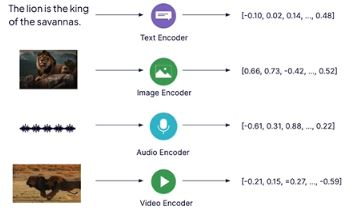
\includegraphics[width=0.5\textwidth]{IMAGES/encode.JPG}
    \caption[Encoding process.]{Encoding process. Source: DeepLearning.AI.\footnotemark.}
    \label{fig:Encoding}
\end{figure}

\footnotetext{\url{https://www.deeplearning.ai/short-courses/building-multimodal-search-and-rag/}}

Thanks to this structure, machine learning techniques can analyze unstructured data, uncover patterns, and generate insights. These techniques are widely applied in fields such as Natural Language Processing (NLP), Computer Vision, Recommendation Systems, and Search Engines. Each application comes with its own challenges. Another key advantage of mathematical vector representations is their ability to facilitate computational efficiency and scalability in data processing.
\section{Dense vs. Sparse Vectors}

It is important to distinguish between two types of vector embeddings: dense and sparse. Dense embeddings have lower dimensionality, with each value carrying meaningful information, while sparse embeddings have high dimensionality but contain only a few non-zero values. Typically, dense vectors are obtained through deep learning techniques or by applying dimensionality reduction to sparse vectors. Each representation has its own strengths, limitations, and use cases, and they can also be effectively combined in certain applications.

\subsubsection{Sparse Vectors}

Sparse embeddings are commonly used in NLP and recommender systems, where data often has high dimensionality but each instance activates only a few features. In a typical sparse vector, each dimension represents a token, and the value indicates that token’s importance within a document. This makes sparse vectors particularly advantageous for applications requiring keyword matching. Several methods exist for creating sparse vectors:

\begin{itemize}
    \item \textbf{Bag of Words (BOW)}: Simple and interpretable, but ignores word order and context.
    \item \textbf{One-Hot Encoding}: Clearly maps each token but results in extremely high dimensionality with large vocabularies.
    \item \textbf{TF-IDF}: Highlights unique terms and relevance within a document but does not capture semantic relationships.
    \item \textbf{BM25}: Extends TF-IDF by considering term frequency and document length but requires full corpus statistics in advance.
    \item \textbf{Sparse Neural Embeddings}: Uses neural networks for efficient keyword matching on large datasets, though often less interpretable than traditional methods.
\end{itemize}

However, sparse vectors struggle to capture nuanced relationships between words. Each dimension may correspond to a word or subword grouping, which aids in interpreting document rankings. Sparse vectors are particularly useful in scenarios with rare keywords or specialized terms that may not appear in standard vocabularies, where general-purpose embeddings might fail to convey the intended meaning. They are highly effective for text search and hybrid search applications.

\subsubsection{Dense Vectors}

Dense embeddings are widely used in NLP and machine learning to capture complex relationships within data. Unlike sparse vectors, dense embeddings represent rich, context-sensitive information in lower-dimensional space, making them ideal for tasks such as semantic search and sentence similarity. While they excel at capturing nuanced meanings, dense embeddings can be computationally intensive and less interpretable. Deep learning techniques are typically used to generate these embeddings, learning from large datasets to uncover intricate patterns. In many cases, dense and sparse vectors can be combined to take advantage of both.

\section{Vector Database Architecture}  

Vector databases share several core components that enable efficient storage, retrieval, and querying of vector embeddings:  

\begin{itemize}  
    \item \textbf{Client Interface}: Provides API or GUI access for querying and managing data.  
    \item \textbf{Query Processor}: Handles similarity searches using distance metrics and ranking mechanisms.  
    \item \textbf{Vector Storage}: Stores vector embeddings and associated metadata.  
    \item \textbf{Indexing Module}: Manages indexing structures to enable efficient retrieval.  
    \item \textbf{Embedding Generation Module}: Converts raw unstructured data (e.g., text, images, audio) into high-dimensional vector embeddings using traditional or deep learning techniques.  
\end{itemize}  
\begin{figure}[h]
    \centering
    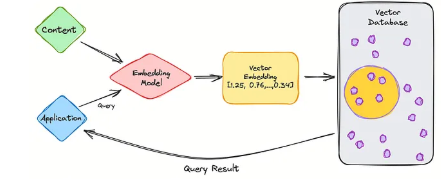
\includegraphics[width=0.6\textwidth]{IMAGES/immagine_2025-02-24_100130378.png}
    \caption[VDB Architecture.]{Architecture. Source: Medium.\footnotemark.}
    \label{fig:Architecture}
\end{figure}
\footnotetext{\url{https://medium.com/data-and-beyond/vector-databases-a-beginners-guide-b050cbbe9ca0}}
\subsection{Querying and Search Efficiency}  
Vector databases balance speed and accuracy using Approximate Nearest Neighbor (ANN) search techniques. These approaches enable efficient retrieval without performing exhaustive comparisons, making them well-suited for large-scale datasets.  

\subsection{Scalability Considerations}  
Handling high-dimensional data efficiently requires scalable solutions. VectorDBs achieve scalability through distributed architectures, memory-efficient indexing, and cloud-based deployments. These capabilities make them viable for both on-premise and large-scale cloud environments.  








\section{Multimodal Vector Space}
One key application of vector DBMSs is the mapping of data in Multimodal Vector Spaces, which refers to the storage and retrieval of data across multiple modalities, such as text, images, audio and video, in a unified embedding space. This means that conceptually related items, regardless of their format (e.g., an image of a lion and the phrase "the king of the jungle"), are placed close to each other in this space.
\begin{figure}[h]
    \centering
    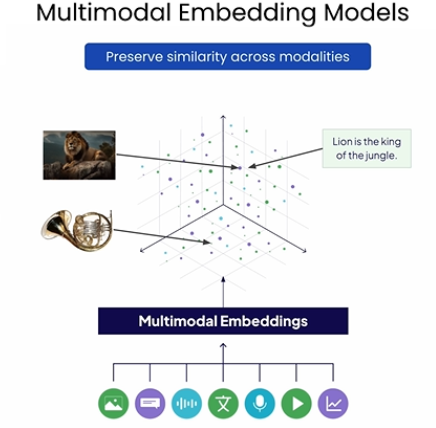
\includegraphics[width=0.5\textwidth]{IMAGES/immagine_2025-02-23_214815401.png}
    \caption{Multimodal Vector Space.}
    \label{fig:multimodal_space}
    \source{\url{https://www.deeplearning.ai/short-courses/building-multimodal-search-and-rag/}}
\end{figure}

The key motivation for multimodal data comes from the fact that humans understand the world, not through a single mode like text alone, but through a combination of sensory inputs. For example, hearing the sound of a cash register can immediately evoke the concept of a store or a purchase. By integrating multiple modalities, we aim to develop systems capable of learning and reasoning across diverse data formats. 
\subsection{Constructing the Multimodal Vector Space}
To achieve this, we employ specialized encoders that learn representations for each modality separately and then align them through contrastive learning.
The process of constructing a Multimodal vector space consists of the following steps:
\begin{enumerate}
    \item Train individual embedding models for each modality (e.g., an image encoder for images, a text encoder for text).
    \item Align these models in a shared vector space.
    \item Optimize the embeddings to ensure cross-modal similarity.
    \item Use contrastive learning to fine-tune the models by distinguishing between positive and negative examples.
\end{enumerate}
\subsection{Applications of Multimodal Retrieval}
Multimodal retrieval has various real-world applications, including:
\begin{itemize}
    \item \textbf{Image-Text Search}: Finding relevant images based on textual queries (e.g., retrieving an image of the Eiffel Tower when searching "Paris landmark").
    \item \textbf{Video Retrieval}: Searching for specific moments in videos using natural language queries.
    \item \textbf{Audio-Visual Understanding}: Associating spoken words with corresponding visual elements in video content.
    \item \textbf{Medical Imaging}: Aligning radiology reports with corresponding X-ray images to enhance diagnostics.
\end{itemize}



\section{Key Products and Features}
The following are leading vector database solutions available in the market:
\begin{itemize}
    \item \textbf{Milvus:} Open-source, distributed database optimized for scalability and GPU acceleration, widely used in AI analytics and recommendation systems.
    \item \textbf{Pinecone:} Managed service with real-time indexing, automatic scaling, and seamless ML integration, ideal for semantic search and anomaly detection.
    \item \textbf{QDrant:} High-performance, open-source vector search engine supporting hybrid search (vector + metadata), multimodality and efficient memory management.
    \item \textbf{Weaviate:} Similar to QDrant offering flexible filtering and retrieval strategies.
\end{itemize}

\chapter{Vectorization Techniques}
In this chapter, we will explore vectorization techniques in depth, beginning with traditional methods such as One-Hot Encoding, Bag of Words, and TF-IDF. We will then transition into fundamental Deep Learning principles, which lay the groundwork for advanced representations, including word embeddings and transformer-based models, enabling richer, context-aware representations. Furthermore Deep Learning principles will serve as context for advanced applications of Vector Databases in the following chapters.

\section{Traditional Vectorization Techniques}
Traditional vectorization techniques transform textual data into numerical representations, enabling computational processing and analysis. These methods primarily rely on statistical properties of text rather than learned representations from deep learning models. This section explores widely used traditional techniques, including One-Hot Encoding (OHE), Bag of Words (BoW), Term Frequency-Inverse Document Frequency (TF-IDF).

\subsection{Tokenization}  
Tokenization is a crucial preprocessing step for both traditional and deep learning-based vectorization. It involves breaking text into smaller units (tokens), with different approaches offering various trade-offs:  

\begin{itemize}  
    \item \textbf{Byte-level tokenization}: Operates on a small vocabulary, encoding text at the byte level.  
    \item \textbf{Word-based tokenization}: Uses full words as tokens, preserving meaning but struggling with unseen words due to a large vocabulary.  
    \item \textbf{Subword tokenization}: A compromise between the two, capturing word roots (e.g., NLP, lemmatization) while remaining trainable and statistically driven.  
\end{itemize}  



\subsection{One-Hot Encoding (OHE)}

One-Hot Encoding (OHE) is the simplest vectorization technique, representing each unique word in a vocabulary as a binary vector. Given a vocabulary of size \( V \), each word \( w_i \) is mapped to a vector of length \( V \) where only the corresponding index is set to 1, while all other elements remain 0. 

For example, given the vocabulary:
\[
\{ \text{apple}, \text{banana}, \text{cherry} \}
\]
the one-hot encoded vectors are:

\[
\text{apple} \rightarrow [1, 0, 0], \quad
\text{banana} \rightarrow [0, 1, 0], \quad
\text{cherry} \rightarrow [0, 0, 1]
\]

Mathematically, for a given word \( w_i \) in a vocabulary of size \( V \), its one-hot representation \( \mathbf{v}_{w_i} \) is:

\begin{equation}
    \mathbf{v}_{w_i} = [0, 0, \dots, 1, \dots, 0, 0]
\end{equation}

where the position of 1 corresponds to the index of the word in the vocabulary.

While simple and interpretable, one-hot encoding suffers from high dimensionality and sparsity, making it inefficient for large vocabularies. Additionally, it does not capture semantic relationships between words (e.g., "cat" and "dog" are equally distant from "fish" in this representation).

\subsection{Bag of Words (BoW)}

The Bag of Words model extends OHE by considering word frequencies in a document rather than binary presence. It represents a document by counting the occurrences of words, ignoring word order and syntax. Formally, let \( D \) be a collection of documents and \( V \) the vocabulary of unique words across all documents. The BoW representation of a document \( d \) is a vector:

\begin{equation}
    \mathbf{v}_d = (f_1, f_2, \dots, f_n)
\end{equation}

where \( f_i \) is the frequency of word \( w_i \) in the document \( d \). While BoW is effective in some applications, it suffers from high dimensionality and lacks semantic understanding.

\subsection{Term Frequency-Inverse Document Frequency (TF-IDF)}

TF-IDF improves upon the BoW model by assigning importance to words based on their frequency across multiple documents. The TF-IDF value for a word \( w \) in a document \( d \) is given by:

\begin{equation}
    \text{TF-IDF}(w, d) = \text{TF}(w, d) \times \text{IDF}(w)
\end{equation}

where:
\begin{itemize}
    \item \textbf{Term Frequency (TF)} measures how frequently a word appears in a document:
    \begin{equation}
        \text{TF}(w, d) = \frac{f_w}{\sum_{w' \in d} f_{w'}}
    \end{equation}
    where \( f_w \) is the count of word \( w \) in document \( d \).

    \item \textbf{Inverse Document Frequency (IDF)} reduces the weight of common words appearing in many documents:
    \begin{equation}
        \text{IDF}(w) = \log \left( \frac{N}{1 + \text{DF}(w)} \right)
    \end{equation}
    where \( N \) is the total number of documents, and \( \text{DF}(w) \) is the number of documents containing \( w \).
\end{itemize}

TF-IDF effectively emphasizes informative words while downplaying common ones, making it useful for tasks like document classification and search retrieval.

\section{Deep Learning}
The conversion of unstructured data to vector embedding is an automatic process that leverages Deep Learning techniques by using Neural Networks, which is essentially a computational model inspired by how the human brain processes information, in a nutshell Neural Networks are composed of layers of interconnected “neurons” that perform calculations on the input data.

\subsection{Neuron}
The “Neuron” is the most basic computational unit of the Neural Network, each neuron takes multiple inputs, each with an associated weight (which indicates the importance), computes their weighted sum, adds a constant called bias, and then passes this result through an activation function, which generates the neuron's output.
\begin{figure}[h]
    \centering
    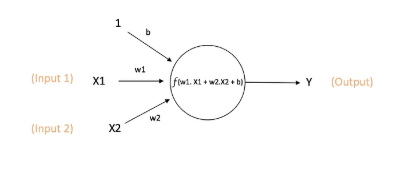
\includegraphics[width=0.6\textwidth]{IMAGES/immagine_2025-02-26_153339240.png}
    \caption[Neuron]{Neuron Source.\footnotemark.}
    \label{fig:Neuron}
\end{figure}
\footnotetext{\url{https://medium.com/analytics-vidhya/neural-networks-in-a-nutshell-bb013f40197d}}

The most popular and widely known activation functions in neural networks are:
\begin{itemize}
    \item \textbf{Sigmoid}: \( \sigma(x) = \frac{1}{1 + e^{-x}} \)
    \item \textbf{Tanh}: \( \tanh(x) = \frac{e^x - e^{-x}}{e^x + e^{-x}} \)
    \item \textbf{ReLU}: \( f(x) = \max(0, x) \)
    \item \textbf{Softmax}: \( \sigma(x_i) = \frac{e^{x_i}}{\sum_{j} e^{x_j}} \)
\end{itemize}

As said before the neural networks is has an architecture that is composed by layers each one with its neurons, they are the following:

\begin{itemize}
    \item \textbf{Input layer}: Which is responsible to receive the input data.
    \item \textbf{Output Layer}: Responsible for producing the final result.
    \item \textbf{Hidden Layer/s}:One or more layers situated between the input and output layers of a neural network, they process and transform the data to help the network learn complex patterns.
\end{itemize}
The number of neurons in each layer and the way they are interconnected depend entirely on the network's design, which is tailored to suit the specific use case.
\subsection{Training process}
Once the neural network architecture is defined, it needs to be trained, which is an iterative process where each iteration called “epoch” is composed of three main steps: Forward propagation, calculation of loss, Backward propagation. The forward propagation starts with initializing the weights and bias (non zero number) and the calculation of the output is done. Then the network's output is compared to the expected result using a loss function. After calculating the loss function, the last step of the iteration is Backward propagation, which through an optimizer adjusts the parameters (weights and biases). The dataset used for training is typically employed in batches, doing so the network trains on each batch on each epoch.


\section{Autoencoders}
One of the architectures used to create vector embeddings leveraging neural networks, is the Autoencoder, a type of neural network with three main parts: encoder layers (which compress the input), a bottleneck layer (where the compact embedding is stored), and decoder layers (which try to rebuild the original input). 
\begin{figure}[h]
    \centering
    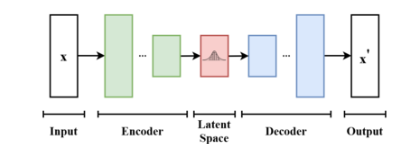
\includegraphics[width=0.6\textwidth]{IMAGES/immagine_2025-02-26_154609390.png}
    \caption[AutoEncoder]{Autoencoder Source.\footnotemark.}
    \label{fig:Autoencoder}
\end{figure}
\footnotetext{\url{https://www.deeplearning.ai/short-courses/building-multimodal-search-and-rag/}}
Basically the encoder layers gradually reduce the number of neurons, compressing the data until it reaches the bottleneck layer. The decoder layers then expand the data again to reconstruct the original input. The vector embedding of the raw data corresponds to the output of the bottleneck layer, and its dimensionality is determined by the number of neurons in that layer. Since the network compresses and decompresses the data, some information is lost in the process, but with proper training the weights will be adjusted to minimize the loss. 
\subsection{Example with the MINST dataset}
As an example, we use the MNIST dataset, which consists of images of handwritten digits. The neural network architecture, shown in the figure below, is an autoencoder with two layers in both the encoder and decoder. The encoder progressively compresses the data from 256 dimensions to 128 and then to 2 dimensions in the bottleneck layer, while the decoder reverses this process to reconstruct the original input. The network uses dense layers, meaning each neuron is fully connected to the neurons in the following layer.
\begin{figure}[h]
    \centering
    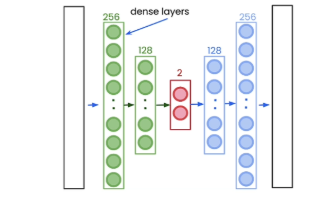
\includegraphics[width=0.6\textwidth]{IMAGES/immagine_2025-02-26_154914801.png}
    \caption[Example of AutoEncoder]{example of AutoEncoder dimensions:
 Source.\footnotemark[3]}
    \label{fig:2D}
\end{figure}
\footnotetext[3]{\url{https://www.deeplearning.ai/short-courses/building-multimodal-search-and-rag/}}

For simplicity and clarity, the images are represented as 2-dimensional vectors, as shown in the plot below.

\begin{figure}[h]
    \centering
    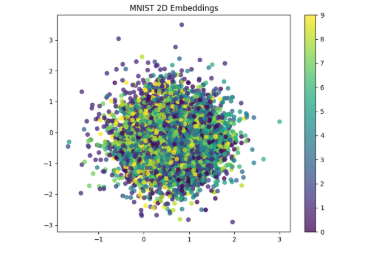
\includegraphics[width=0.6\textwidth]{IMAGES/immagine_2025-02-26_155006209.png}
    \caption[MNIST 2D]{MNIST mapped in 2D:
 Source.\footnotemark[3]}
    \label{fig:2D}
\end{figure}


As expected, some information is lost during the compression process, as the input and output images are not identical. However, by adjusting the weights, the network can minimize this loss and produce outputs closer to the original.
\begin{figure}[h]
    \centering
    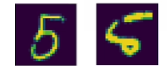
\includegraphics[width=0.6\textwidth]{IMAGES/immagine_2025-02-26_155109338.png}
    \caption[MNIST Results]{Before and After encoding:
 Source.\footnotemark[3]}
    \label{fig:2D}
\end{figure}

In the context of VectorDBs, the encoder is the more relevant component, as it outputs the embeddings needed for database operations. Embeddings can be produced by pre-trained or use-case specific models in order to capture insights.
As shown above, it’s easy for a person to recognize that the first two images represent the same entity. Thanks to the mathematical properties of embeddings, we can make this relationship machine-understandable. By using a similarity function, the system can also determine which pairs of images are more similar
\section{Evolution to Context aware techniques}
While autoencoders provide a compressed representation of the data, and can be trained in an unsupervised way, they still require a training dataset and do not capture contextual relationships. For these reasons, next step mechanisms of that capture the contextual dependencies have been developed such as Recurrent Neural Networks (RNNs) and Long Short-Term Memory Networks (LSTMs), which we will briefly show their functionalities and how they paved the way to Transformers.

\subsection{Recurrent Neural Networks (RNNs)}

Recurrent Neural Networks (RNNs) introduced the idea of modeling sequential dependencies by maintaining a hidden state \( h_t \) that evolves over time:

\begin{equation}
    h_t = f(W_h h_{t-1} + W_x x_t + b),
\end{equation}

where \( W_h \) and \( W_x \) are weight matrices, \( b \) is a bias term, and \( f \) is an activation function (e.g., tanh or ReLU). However, RNNs suffer from the \textit{vanishing gradient problem}, meaning that the gradient the derivative of the loss function, which provides information information of the direction that the model is taking, becomes very small during backpropagation, making it difficult to learn long-range dependencies.
\subsection{LSTM}
LSTMs (Long Short-Term Memory networks) improve upon standard RNNs (Recurrent Neural Networks) by introducing a \textbf{memory cell} \( C_t \) and \textbf{gating mechanisms} that control the flow of information over time. This allows the network to "remember" important information for longer periods and "forget" irrelevant data.
At each time step \( t \), the LSTM takes the input \( x_t \) and the previous hidden state \( h_{t-1} \), and updates the memory cell \( C_t \) and hidden state \( h_t \). The LSTM consists of the following components:

\begin{itemize}
    \item The \textbf{forget gate} \( f_t \) decides how much of the previous memory \( C_{t-1} \) should be kept.
    \item The \textbf{input gate} \( i_t \) controls how much new information \( \tilde{C}_t \) should be added to the memory cell.
    \item The \textbf{output gate} \( o_t \) decides what part of the memory cell \( C_t \) should be output as the current hidden state \( h_t \).
\end{itemize}

The memory cell is updated as follows:

\[
C_t = f_t \odot C_{t-1} + i_t \odot \tilde{C}_t
\]

where \( \tilde{C}_t \) is the candidate memory, computed from the input \( x_t \) and previous hidden state \( h_{t-1} \). The hidden state is then computed as:

\[
h_t = o_t \odot \tanh(C_t)
\]
\subsection{The Transformer Architecture}
Transformers address LSTMs' scalability issues by processing entire sequences simultaneously using self-attention, the core mechanism of the architecture. Self-attention allows the model to interpret a word’s meaning based on its context, even when the same word has different meanings. The self-attention mechanism computes attention scores as:
\begin{equation}
A = \frac{QK^T}{\sqrt{d_k}}
\end{equation}
where  are the query, key, and value matrices derived from input embeddings. Specifically:
\begin{itemize}
\item  \textbf{Q}(Query): Represents the current word/token for which attention is being computed.
\item  \textbf{K}(Key): Represents all words/tokens in the sequence, determining relevance.
\item  \textbf{V}(Value): Contains the actual token representations used to construct the final weighted output.
\end{itemize}
These matrices are obtained by linearly transforming the input embeddings using learned weight matrices :
\begin{equation}
Q = X W_Q, \quad K = X W_K, \quad V = X W_V.
\end{equation}
The attention scores are normalized using softmax and then we compute the final representation with V:
\begin{equation}
    Z = \text{softmax}\left( \frac{QK^T}{\sqrt{d_k}} \right)V.
\end{equation}
Multi-head attention enhances this mechanism by capturing multiple representation aspects, each attention head processes the input independently with learned projections:  
\[
\text{head}_i = \text{Attention}(Q W_i^Q, K W_i^K, V W_i^V),
\]  
where \( W_i^Q \), \( W_i^K \), and \( W_i^V \) are learned projection matrices for queries, keys, and values, respectively. The outputs of all \( h \) heads are concatenated and linearly transformed using another learned weight matrix \( W^O \):  
\[
\text{MultiHead}(Q, K, V) = \text{Concat}(\text{head}_1, \dots, \text{head}_h) W^O.
\]  
Here, \( W^O \) ensures that the final output maintains the desired dimensionality for subsequent layers.
\subsubsection{GPT: Autoregressive Transformer Models}  
The Generative Pre-trained Transformer (GPT) series, along with models like Mistral and LLaMA 2, follows an \textbf{autoregressive} architecture, predicting one token at a time based on prior tokens:  
\begin{equation}
    P(x_t | x_1, x_2, ..., x_{t-1})
\end{equation}  
GPT uses \textbf{causal self-attention}, ensuring tokens only attend to past inputs, making it effective for text generation. It is trained unsupervised on vast text corpora using next-token prediction. During training, a prompt like \textit{"Jack and Jill went over..."} leads the model to assign probabilities to possible next tokens. Training involves guiding initial tokens (e.g., forcing \textit{"The Rock"} for \textit{"The rock at first..."}) and continuing until reaching a token limit or an \texttt{[EOS]} token.  
\begin{figure}[h]
    \centering
    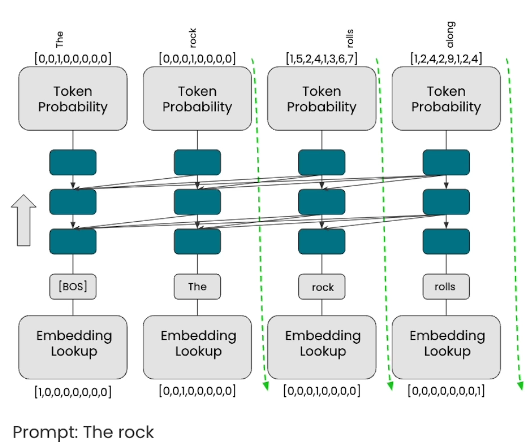
\includegraphics[width=0.4\textwidth]{IMAGES/immagine_2025-02-26_110808787.png}
    \caption[GPT]{GPT model example. Source: DeepLearning.AI.\footnotemark.}
    \label{fig:GPT model}
\end{figure}
\footnotetext{\url{https://www.deeplearning.ai/short-courses/building-multimodal-search-and-rag/}}
\subsection{Visual Transformers (ViTs)}

Visual Transformers extend the principles of self-attention, initially designed for textual data, to computer vision tasks. A Vision Transformer (ViT) processes an image by dividing it into patches, embedding each patch, and applying a transformer model to classify the image based on its patch representations.

\begin{figure}[h]
    \centering
    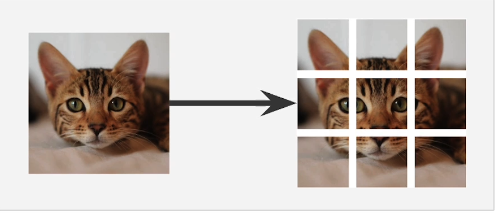
\includegraphics[width=0.4\textwidth]{IMAGES/immagine_2025-02-26_112843716.png}
    \caption[Image Patching]{Image patching. Source: DeepLearning.AI.\footnotemark[4]}
    \label{fig: Patching }
\end{figure}

Key steps in ViT include:

\begin{itemize}
    \item \textbf{Patch Embedding}: An input image of size \( H \times W \) is divided into non-overlapping patches of size \( P \times P \), flattened, and projected into an embedding space.
    \item \textbf{Positional Encoding}: Added to embeddings to retain spatial information.
    \item \textbf{Multi-Head Self-Attention}: Computes relationships across patches.
    \item \textbf{Classification Head}: Uses a CLS token for final classification.
\end{itemize}

\begin{figure}[h]
    \centering
    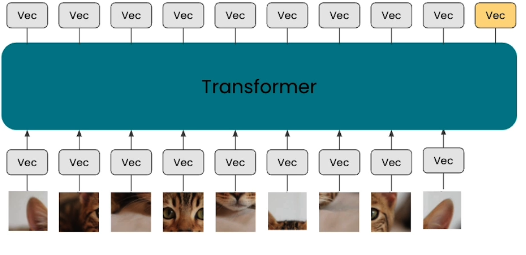
\includegraphics[width=0.4\textwidth]{IMAGES/immagine_2025-02-26_112630864.png}
    \caption[Vision Transformer]{Vision Transformer process. Source: DeepLearning.AI.\footnotemark[4]}
    \label{fig:Vi Transformer }
\end{figure}
\footnotetext[4]{\url{https://www.deeplearning.ai/short-courses/building-multimodal-search-and-rag/}}

\section{Training LLMs to See Images and Multimodality}
Recent advancements in multimodal learning have enabled Large Language Models (LLMs) to not only process text but also understand and generate responses based on visual inputs. One key approach to achieve this is \textbf{Visual Instruction Tuning}. In this process, an LLM is trained to take both visual and textual inputs, allowing it to generate appropriate responses to prompts that involve both types of data. For instance, when given an image of a painting and a prompt like "Who drew this painting?", the model can correctly respond with "Vincent Van Gogh."

\subsection{Multimodal Learning Process}
Large Language Models can be trained to process visual and language input, the process starts with patching and embedding the images as shown before. Moreover, the text prompt is also embedded in a vector space. The model then processes these embeddings, representing both visual and textual information. The core of the model’s training involves integrating these two types of embeddings—\textit{visual embeddings} (from image patches) and \textit{language embeddings} (from text). This allows the model to consider both image and text inputs when generating a response, making it capable of handling Multimodal requests.
\begin{figure}[h]
    \centering
    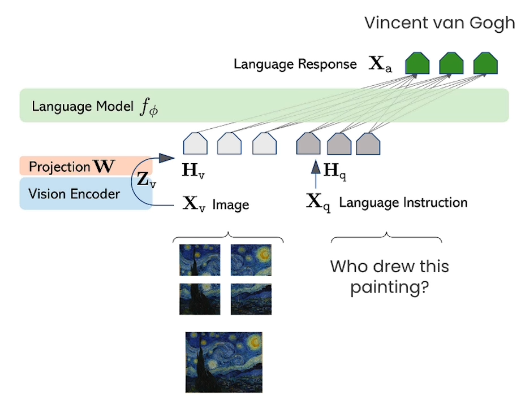
\includegraphics[width=0.6\textwidth]{IMAGES/immagine_2025-02-26_113532424.png}
    \caption[Text and Image input processed]{Text and Image input processed. Source: DeepLearning.AI.\footnotemark[4]}
    \label{fig:InputText}
\end{figure}
The resulting model can handle tasks that require both visual understanding and language generation, such as identifying objects in an image or answering questions about visual content.

\subsection{Large Multimodal Models (LMMs)}
\textbf{Large Multimodal Models (LMMs)} take this integration even further by combining multiple types of data—text, images, audio, and video—into a single model. These models extend the capabilities of traditional LLMs by processing and understanding a wider range of inputs, which enables more sophisticated, context-aware AI systems.

\subsection{Key Components of Multimodal Learning}

Multimodal learning is the process of combining and aligning different types of data to produce richer and more meaningful representations. The main components of LMMs include:

\begin{itemize}
    \item \textbf{Modality-Specific Encoders}: Each modality (e.g., text, image, audio) is processed by a dedicated encoder. For example, in CLIP (Contrastive Language-Image Pretraining), distinct encoders handle the text and image inputs, learning a shared embedding space that links the two modalities.
  
    \item \textbf{Cross-Attention Mechanisms}: These mechanisms allow the model to exchange information between different modalities, enhancing the model's understanding of the data. For example, this helps the model connect visual features with corresponding textual descriptions.
  
    \item \textbf{Unified Representations}: The model fuses the multimodal inputs into a single vector space, facilitating tasks like generation and retrieval that require understanding and synthesizing information across modalities.
\end{itemize}

\subsection{Contrastive Learning for Multimodal Embeddings}
Contrastive learning plays a key role in aligning embeddings from different modalities. The goal is to learn a representation where similar data points (positive pairs) are drawn closer together, while dissimilar ones (negative pairs) are pushed further apart.
\subsubsection{Contrastive Learning Procedure}
The contrastive learning process follows these steps:
\begin{enumerate}
    \item Define an anchor (e.g., an image of a cat).
    \item Identify a positive example, which is semantically related to the anchor (e.g., the phrase "a small feline").
    \item Identify a negative example, which is unrelated to the anchor (e.g., an image of a car).
    \item Train the model to minimize the distance between the anchor and the positive example while maximizing the distance to the negative example.
\end{enumerate}

\begin{figure}[h]
    \centering
    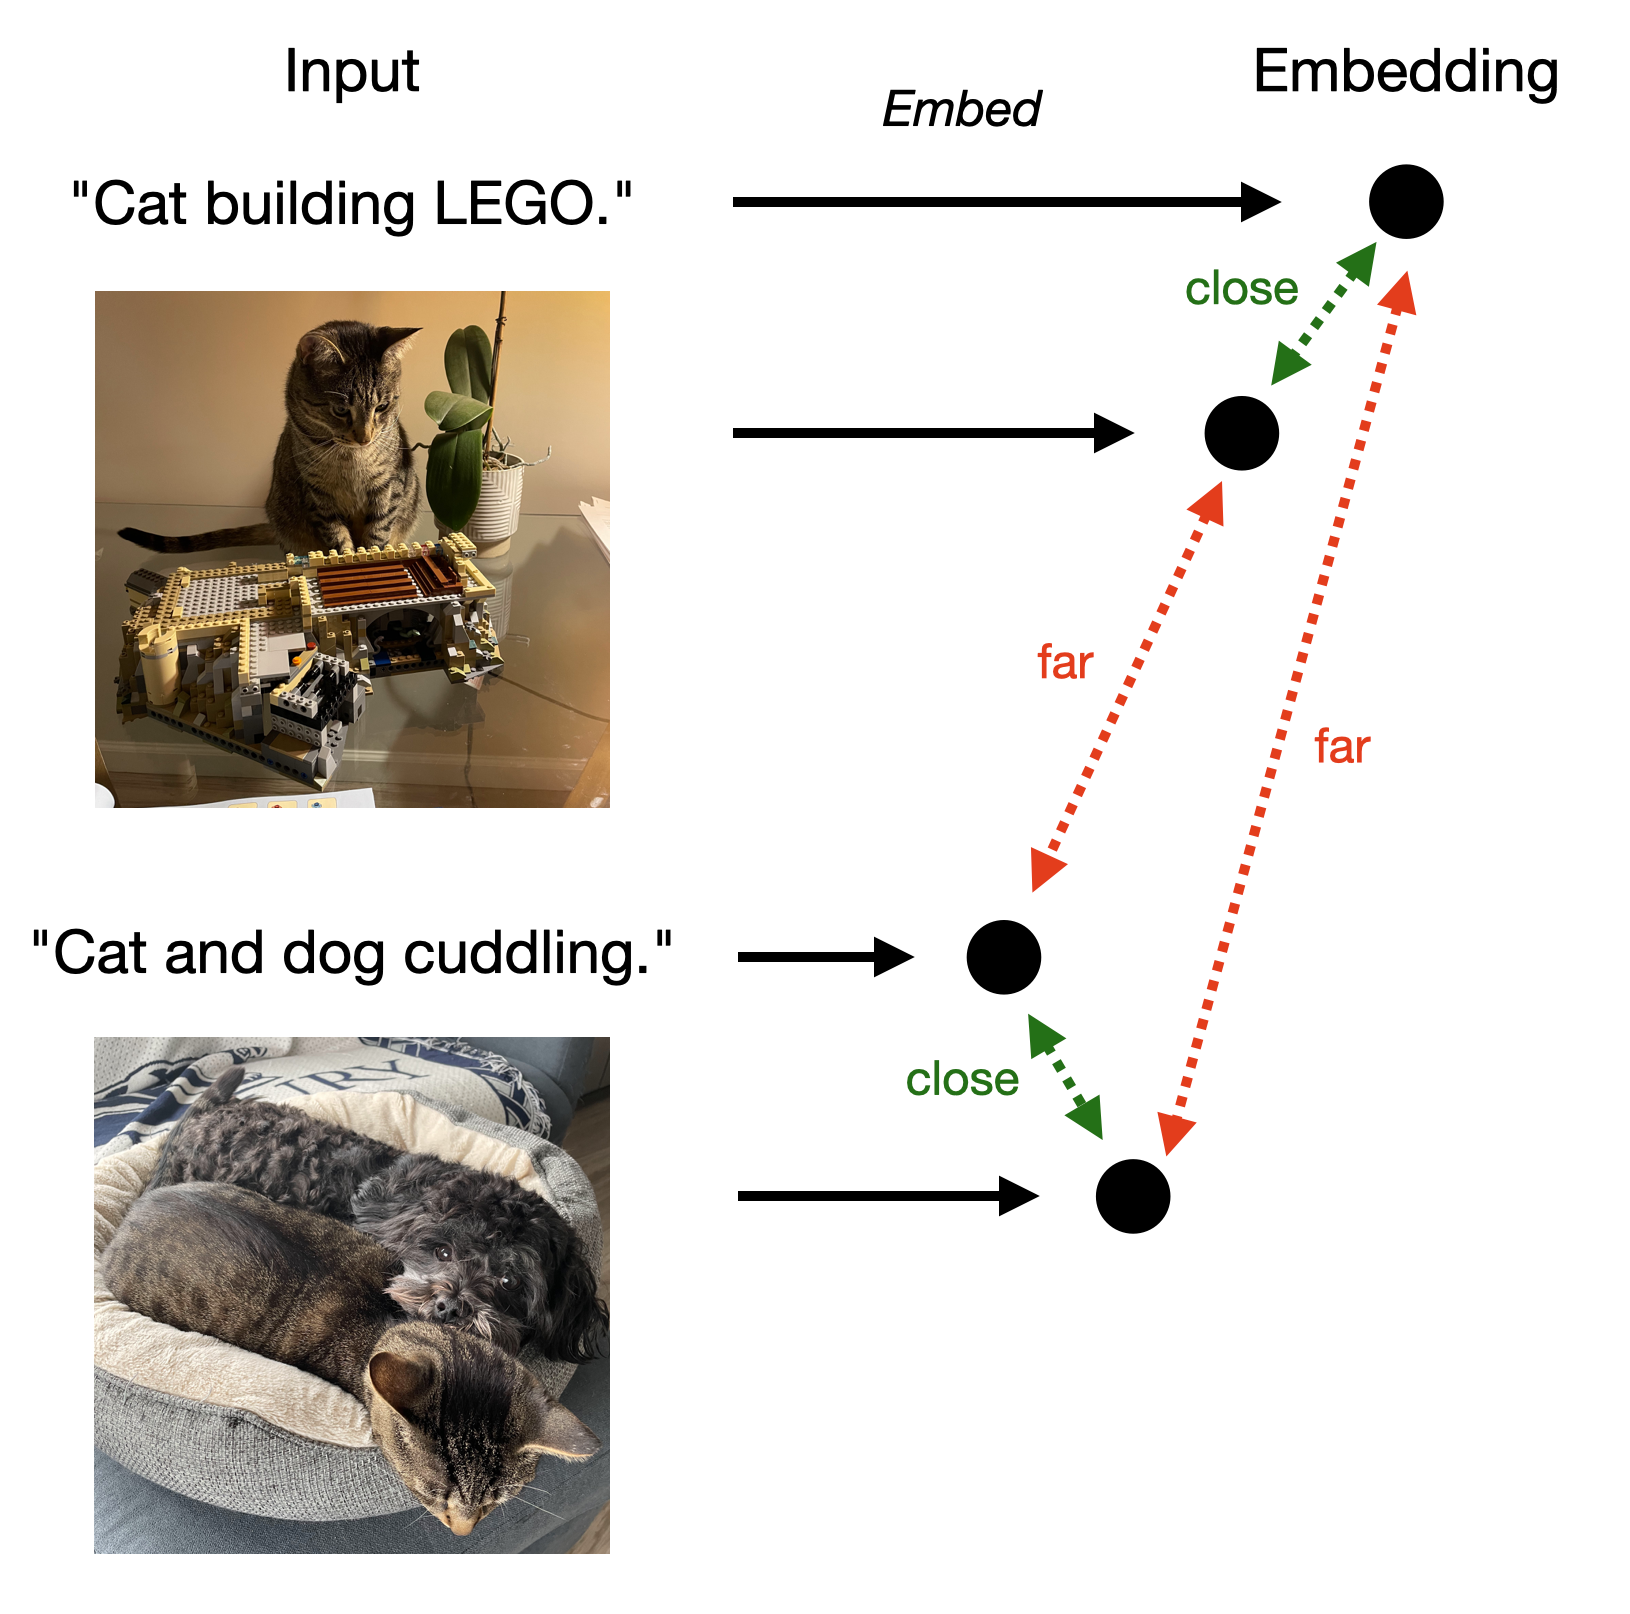
\includegraphics[width=0.55\textwidth]{IMAGES/contrastive_CLIP.png}
    \caption[Illustration of Contrastive Learning]{Illustration of Contrastive Learning. Source:v7labs\footnotemark.}
    \label{fig:contrastive_learning}
\end{figure}
\footnotetext{\url{https://www.v7labs.com/blog/contrastive-learning-guide}}
\subsubsection{Contrastive Loss Function}
The contrastive loss function is formulated as follows:

\begin{equation}
\mathcal{L} = -\log \frac{\exp(\text{sim}(q, k^+))}{\sum_{k \in K} \exp(\text{sim}(q, k))}
\end{equation}
where:
\begin{itemize}
    \item \( q \) is the embedding of an anchor (e.g., an image encoded by a function \( f \)).
    \item \( k^+ \) is the embedding of a positive example (e.g., a corresponding text encoded by function \( g \)).
    \item \( K \) includes both the positive example and a set of negative examples \( k^- \).
    \item \( \text{sim}(q, k) \) denotes a similarity measure, such as cosine similarity.
    \item The negative log ensures that the similarity between \( q \) and \( k^+ \) is maximized while pushing away the negative examples \( k^- \).
\end{itemize}
